%!TEX root = ../../../adrien_gomar_phd.tex

The outlet isentropic Mach number is $0.99$ for an inlet Mach number of $0.4$. 
This case, for which experimental uncertainties are available, 
has been largely addressed in the literature by
\citet{Sbardella2001,Duta2002,Campobasso2003,Cinnella2004} and \citet{Huang2013a}. 
This test case is challenging in terms of non-linearities as a separation bubble and a shock are present.

\paragraph{Steady results}

Steady results of the isentropic Mach number are shown in
Figure~\ref{fig:stcf11_rans_transonic}.  For this flow regime,
a small separation
bubble develops on the suction side at the leading edge.  
The flow then accelerates, followed by a shock.  
The experimental data suggests that the shock appears
sooner on the suction side than in the computations; all the results 
reported in the literature exhibit similar discrepancies (see
Refs.~\cite{Fransson1999,Sbardella2001,Duta2002,Campobasso2003,Cinnella2004,Huang2013a}). 
Otherwise, the present results are in fair agreement with experimental data.
\begin{figure}[htp]
  \centering
  \subfigure[isentropic Mach number at blade walls]{
  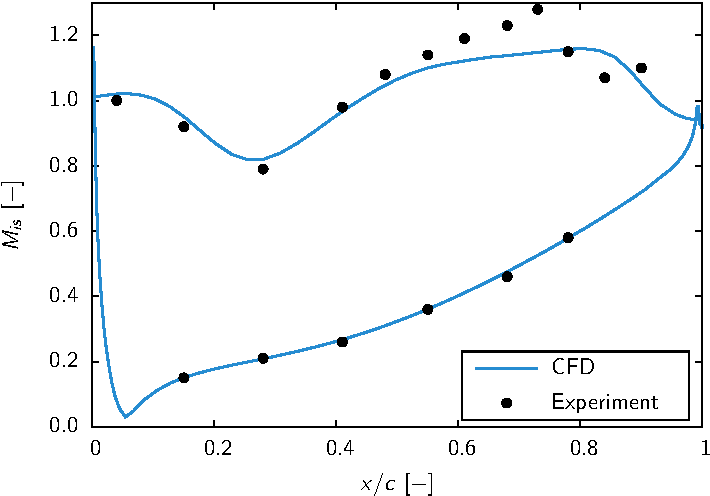
\includegraphics[height=.3\textwidth]{STCF11_RANS_TRANSONIC_PPT.pdf}}
  \subfigure[contours of static pressure with streamlines]{
  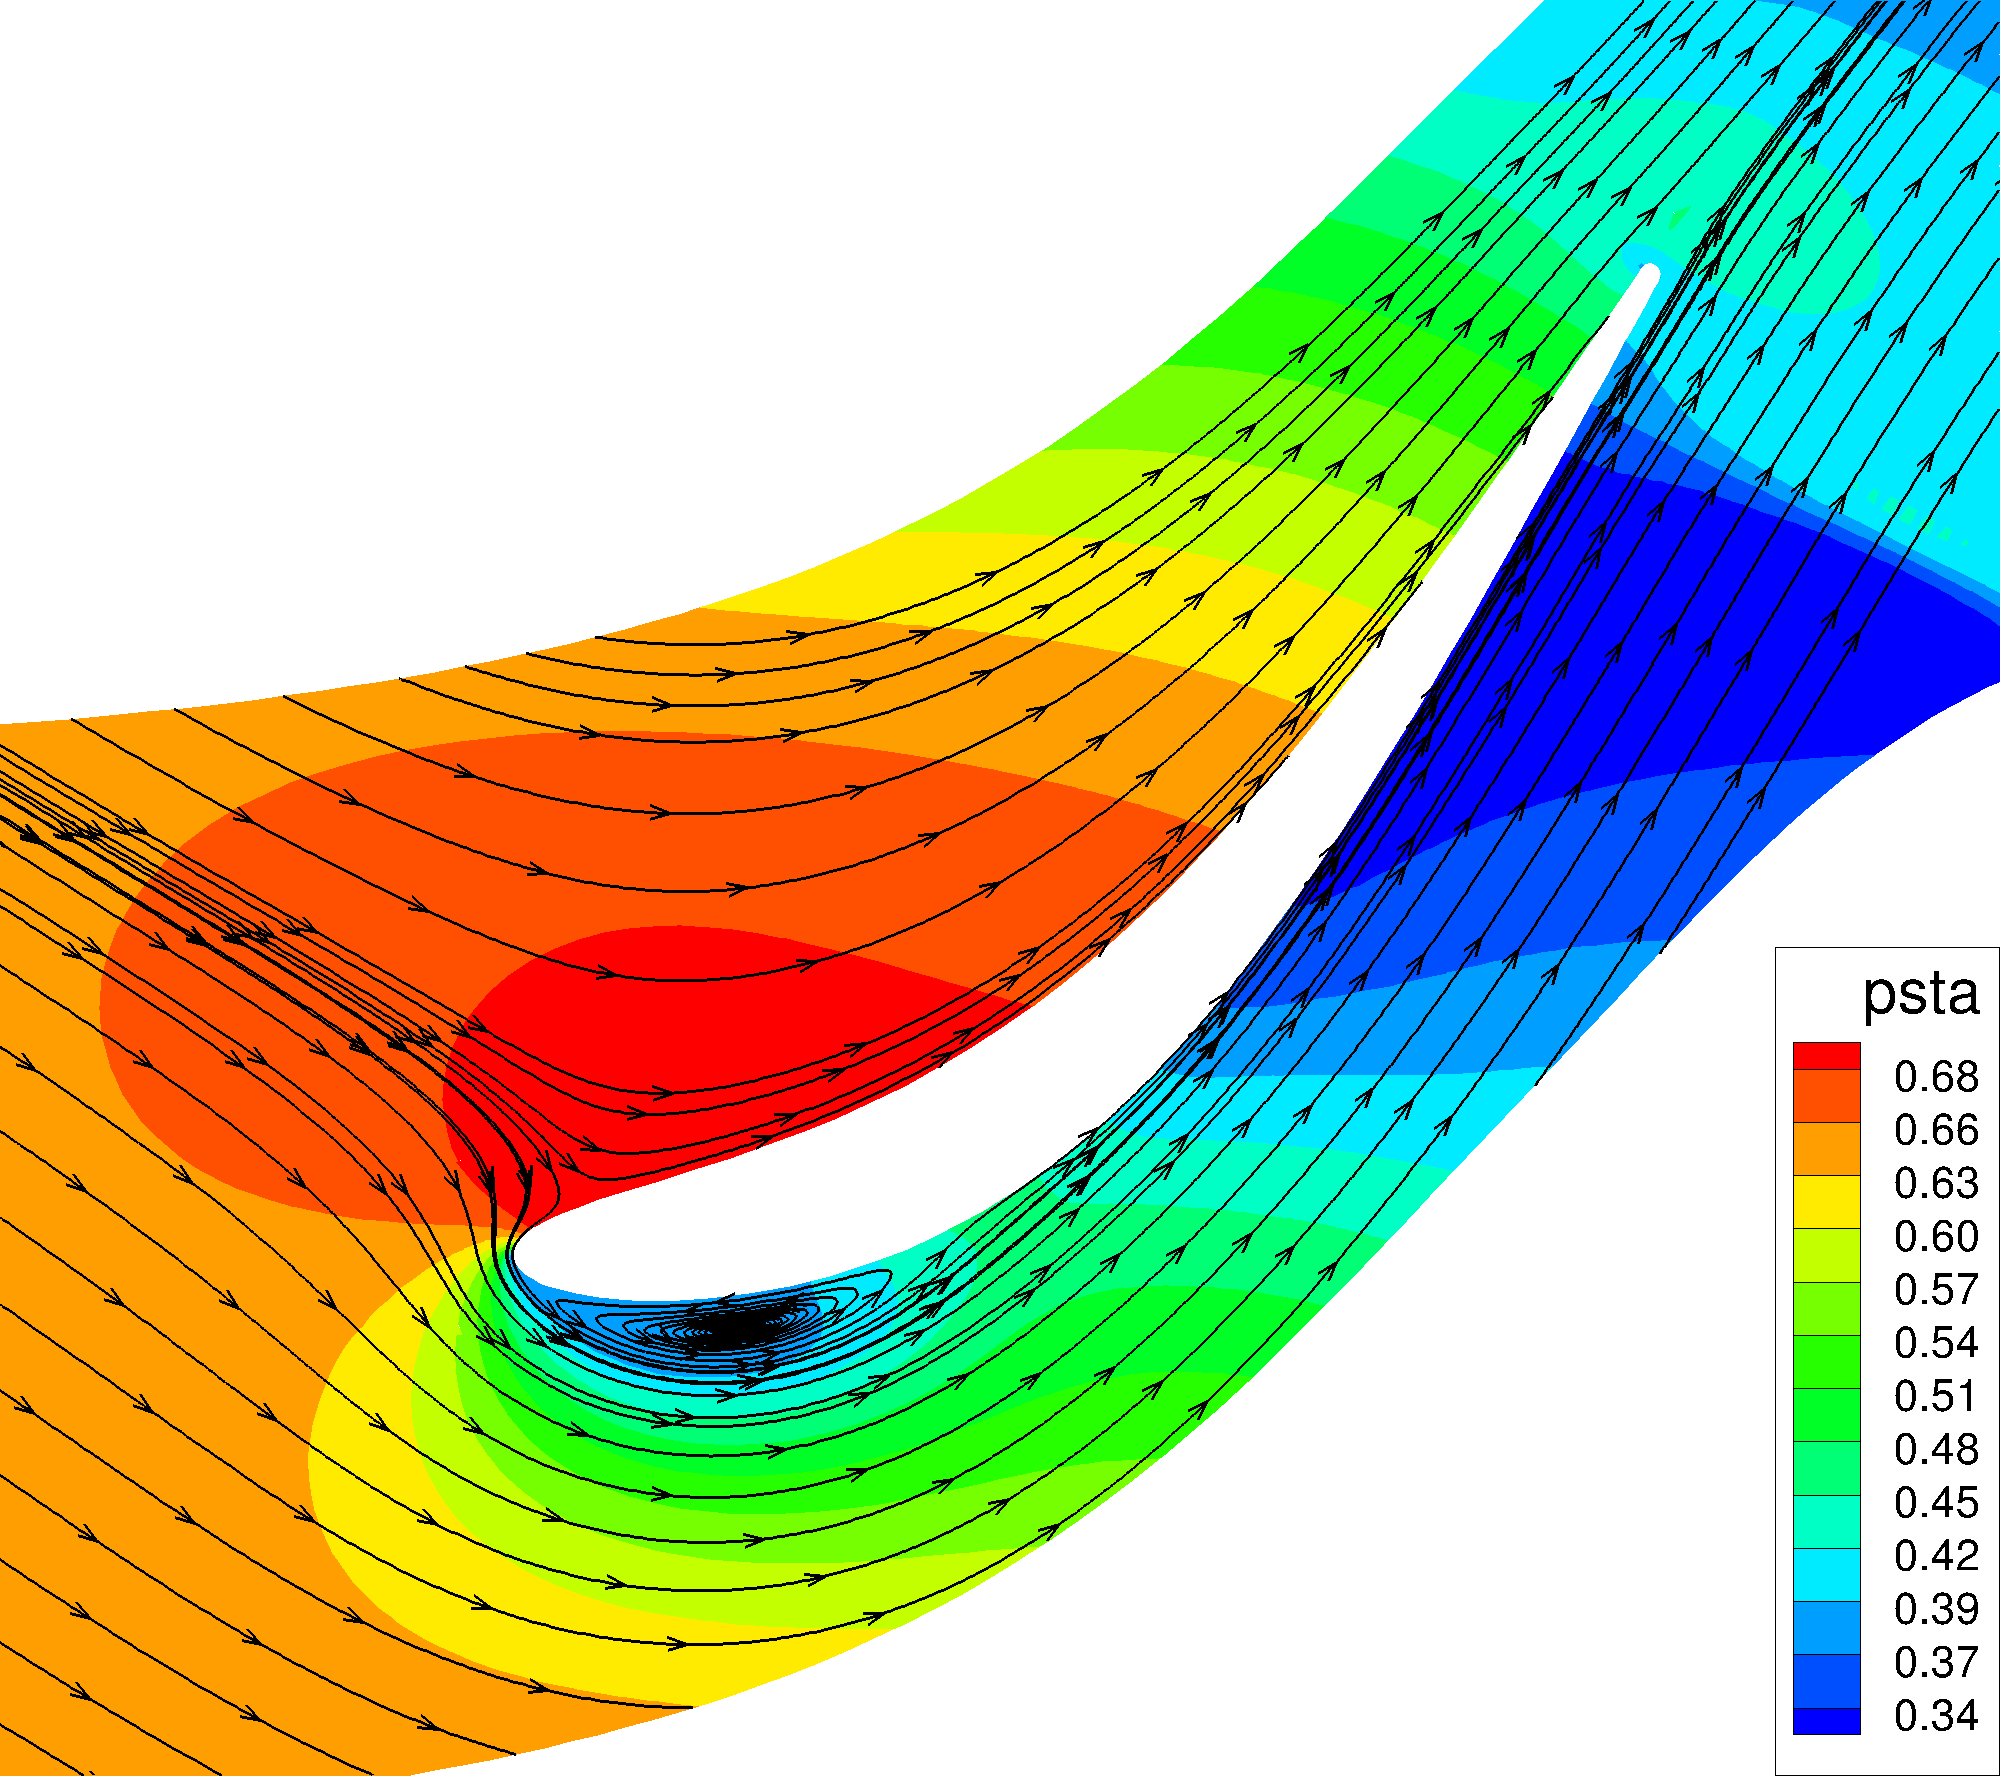
\includegraphics[height=.3\textwidth]{stcf11_transonic_local.png}}
  \caption{Steady results for the STCF~11 configuration, transonic case.}
  \label{fig:stcf11_rans_transonic}
\end{figure}

\paragraph{Aeroelastic results}

% unsteady results
The aeroelastic experimental data are compared to the present results
obtained with both the DTS and the HB approach.  
Considering the opposite phase vibration case (the 10\textsuperscript{th} nodal diameter), 
the amplitude and the
phase of the pressure coefficient are presented in
Figure~\ref{fig:stcf11_ael_transonic_ibpa_180_paper}. Also plotted are the results of
\citet{Cinnella2004}, computed with a non-linear viscous
approach using the Spalart-Allmaras turbulence model. The present HB and the DTS
results are superimposed, which indicates that the one harmonic HB solution is able
to reproduce the unsteady non-linear effects without increasing the
number of harmonics. The results are in good agreement with
the experimental data and display the same trends as that of
\citet{Cinnella2004}. A slight discrepancy can be observed within the shock
region, where the amplitude and the phase phenomena are predicted
further than the experiments indicate.  This can be attributed to the poor
prediction of the shock position (indicated in 
Figure~\ref{fig:stcf11_rans_transonic}) and thus the poor prediction
of its interaction with the motion of the blade.
\begin{figure}[htp]
  \centering
  \subfigure[amplitude]{
  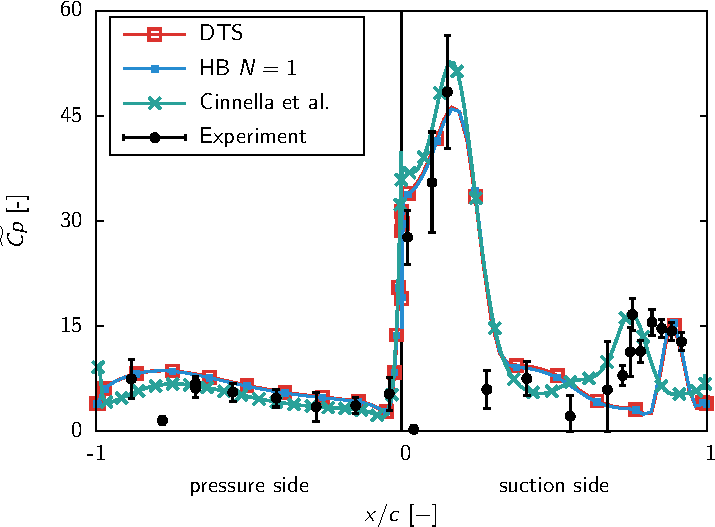
\includegraphics[width=.45\textwidth]{STCF11_AEL_TRANSONIC_IBPA_180_Cp_ppt.pdf}}
  \subfigure[phase]{
  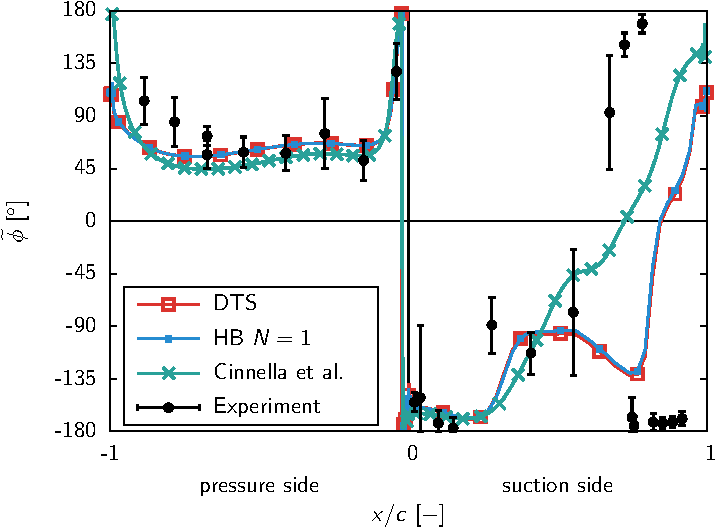
\includegraphics[width=.45\textwidth]{STCF11_AEL_TRANSONIC_IBPA_180_Phi_ppt.pdf}}
  \caption{Wall pressure harmonic analysis for an opposite phase vibration, transonic case.}
  \label{fig:stcf11_ael_transonic_ibpa_180_paper}
\end{figure}

The results for the $-2$\textsuperscript{nd} nodal diameter are also shown in
Figure~\ref{fig:stcf11_ael_transonic_ibpa_324_paper}. Again,
the HB results are superimposed with the DTS ones. Moreover, these are in
good agreement with the experiments, considering the uncertainties of
the experimental data.
\begin{figure}[htp]
  \centering
  \subfigure[amplitude]{
  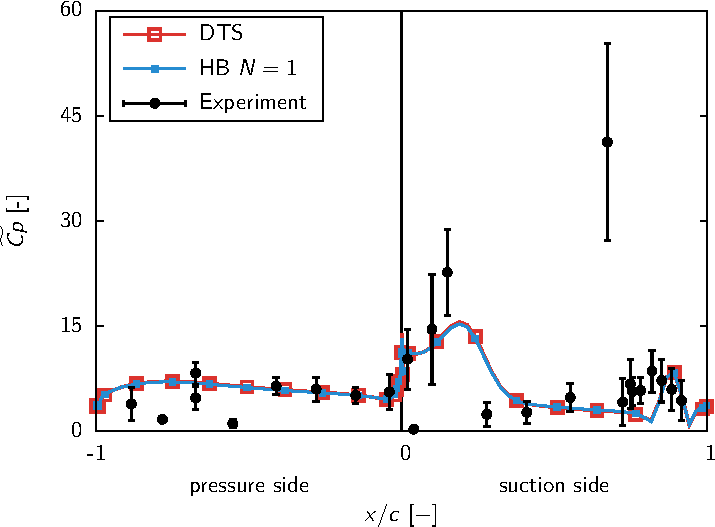
\includegraphics[width=.45\textwidth]{STCF11_AEL_TRANSONIC_IBPA_324_Cp_ppt.pdf}}
  \subfigure[phase]{
  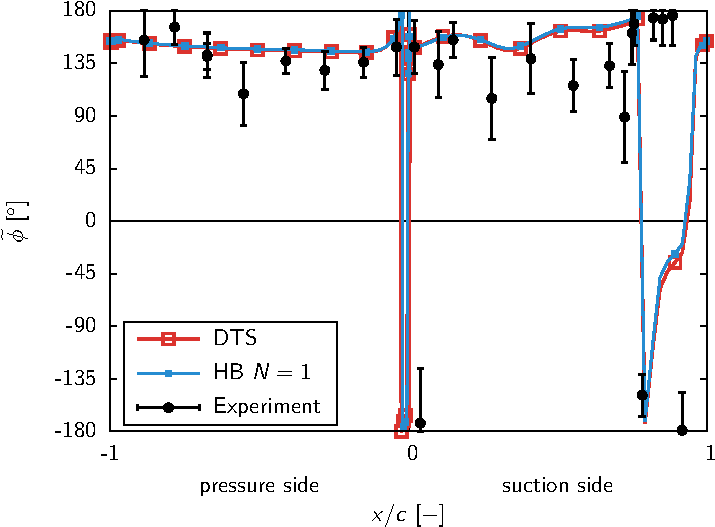
\includegraphics[width=.45\textwidth]{STCF11_AEL_TRANSONIC_IBPA_324_Phi_ppt.pdf}}
  \caption{Wall pressure harmonic analysis for \mbox{$n_d=-2$}, transonic case.}
  \label{fig:stcf11_ael_transonic_ibpa_324_paper}
\end{figure}

Let us clarify one important thing here: 
the convergence of the harmonic balance approach depends
on the smoothness of the temporal phenomenon.
This effect can be emphasized by two 
aeroelastic computations that have been performed 
using a harmonic balance approach. 
The first one is the case of 
an airfoil with an oscillating 
flap~\cite{JDufour2009}. In this simulation, the flap is oscillating
under transonic inflow conditions, resulting in a shock swinging temporally
back and forth from the pressure side to the
suction side. As the discontinuity is
both spatial (a shock is seen on the field) and temporal
(this shock is moving with respect to time), the number
of harmonics needed to capture this phenomenon was high ($N=3$). This is
consistent with the capturing of a rectangular function
as shown in Sec.~\ref{cha:limitations_convergence}.
Contrarily, a recent publication~\cite{Huang2013a} and the
current results on the validation
of the use of harmonic balance approach to predict
aeroelasticity damping within turbomachinery, have highlighted
different conclusions. Under the first bending mode
of the blade, the shock remains steady in the relative bending frame
of reference. As the shock
is only spatial, both authors show a convergence of 
harmonic balance approach with only $N=1$ harmonic. Thus, if the shock
structure is only spatial, Fourier-based time methods will not need
extra harmonics to converge, while for a temporally moving discontinuity
(which is not our case here), the number
of harmonics to converge will be higher.

The damping is shown in Figure~\ref{fig:stcf11_transonic_damping} for
the transonic case. Also plotted are the results from
\citet{Fransson1999} (potential code), and 
from \citet{Cinnella2004} (RANS). The scattering is much more severe
than for the subsonic case. The trends obtained with the RANS approaches are similar. However, the
discrepancies between the two RANS codes are significant in terms of
levels.
Recently, \citet{Vogt2011} reported similar discrepancies 
for damping predictions of subsonic and transonic cascades, 
showing that the damping can be significantly affected by 
small local changes in the amplitude or the phase.
\begin{figure}[htp]
  \centering
  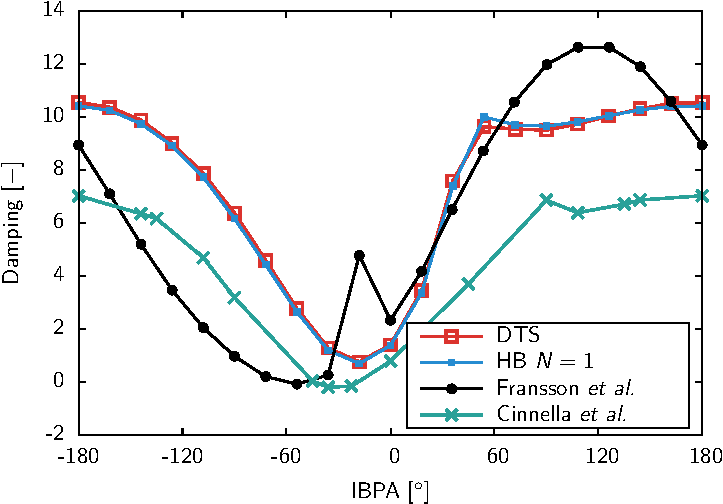
\includegraphics[width=.45\linewidth]{STCF11_TRANSONIC_DAMPING_PPT.pdf}
  \caption{Aerodynamic damping coefficient versus IBPA, transonic case.}
  \label{fig:stcf11_transonic_damping}
\end{figure}

In terms of computational efficiency, the HB method is 7 times faster
than the DTS for all the IBPAs which is very good considering 
that the DTS computations
were done using chorochronic boundary conditions which already
provides computational savings compared to a
full $360^\circ$ simulation.